\let\negmpace\undefined
\let\negthickspace\undefined
\documentclass[journal]{IEEEtran}
\usepackage[a5paper, margin=10mm, onecolumn]{geometry}
%\usepackage{lmodern} % Ensure lmodern is loaded for pdflatex
\usepackage{tfrupee} % Include tfrupee package
\setlength{\headheight}{1cm} % Set the height of the header box
\setlength{\headsep}{0mm}     % Set the distance between the header box and the top of the text
\usepackage{xparse}
\usepackage{romannum}
\usepackage{gvv-book}
\usepackage{gvv}
\usepackage{cite}
\usepackage{amsmath,amssymb,amsfonts,amsthm}
\usepackage{algorithmic}
\usepackage{graphicx}
\usepackage{textcomp}
\usepackage{xcolor}
\usepackage{txfonts}
\usepackage{listings}
\usepackage{enumitem}
\usepackage{mathtools}
\usepackage{gensymb}
\usepackage{comment}
\usepackage[breaklinks=true]{hyperref}
\usepackage{tkz-euclide} 
\usepackage{listings}
% \usepackage{gvv}                                        
\def\inputGnumericTable{}                                 
\usepackage[latin1]{inputenc}                                
\usepackage{color}   
\usepackage{amsmath}
\usepackage{array}                                            
\usepackage{longtable}                                       
\usepackage{calc}                                             
\usepackage{multirow}                                         
\usepackage{hhline}                                           
\usepackage{ifthen}                                           
\usepackage{lscape}
\renewcommand{\thefigure}{\theenumi}
\renewcommand{\thetable}{\theenumi}
\setlength{\intextsep}{10pt} % Space between text and floats
\numberwithin{equation}{enumi}
\numberwithin{figure}{enumi}
\renewcommand{\thetable}{\theenumi}
\begin{document}
\bibliographystyle{IEEEtran}
\title{2007-ME-35 to 51}
\author{EE24BTECH11038 - MALAKALA BALA SUBRAHMANYA ARAVIND}
% \maketitle
% \newpage
% \bigskip
{\let\newpage\relax\maketitle}
\begin{enumerate}[start=35]
\item A building has to be maintained at 21$\degree\brak{\text{dry bulb}}$ and 14.5$\degree \brak{\text{wet bulb}}$. The dew point temperature under these conditions is 10.17$\degree$. The outside temperature is -23$\degree\brak{\text{dry bulb}}$ and the internal and external surface heat transfer coefficients are 8 $w/m^2k$ and 23 $w/m^2k$ respectively. If the building wall has a thermal conductivity of 1.2 $w/mk$, the minimum thickness $\brak{\text {in m}}$ of the wall required to prevent condensation is:
\begin{enumerate}
    \item 0.471
    \item 0.407
    \item 0.321
    \item 0.125
\end{enumerate}
\bigskip
\item Atmospheric air at a flow rate of 3 Kg/s $\brak{\text{on dry basis}}$, enters a cooling and dehumidifying coil with an enthalpy of 85 kJ/kg of dry air and a humidity ratio of 19 grams/kg of dry air. The air leaves the coil with an enthalpy of 43 kJ/kg of dry air and a humidity ratio of  grams/Kg of dry air. If the condensate water leaves the coil with an enthalpy of 67 kJ/kg, the required cooling capacity of the coil in kW is:
\begin{enumerate}
    \item 75
    \item 123.8
    \item 128.2
    \item 159.0
\end{enumerate}
\bigskip
\item A heat transformer is a device that transfers a part of the heat, supplied to it at an intermediate temperature, to a high temperature reservoir while rejecting the remaining part to a low temperature heat sink. In such a heat transformer, 100 kJ of heat is supplied at 350 K. The maximum amount of heat in kJ that can be transferred to 400 K, when the rest is rejected to a heat sink at 300 K is:
\begin{enumerate}
    \item 12.5
    \item 14.29
    \item 33.33
    \item 57.14
\end{enumerate}
\bigskip
\item Which combination of the following statements is correct?\\
The incorporation of reheater in a steam power plant:\\
P: always increases the thermal efficiency of the plant.\\
Q: always increases the dryness fraction of steam at condenser inlet.
\begin{enumerate}
    \item P only
    \item Q only
    \item both P and Q only
    \item neither P nor Q
\end{enumerate}
\bigskip
\item Which combination of the following statements is correct?\\
P: A gas cools upon expansion only when its Joule-Thomson coefficient is positive in the temperature range of expansion.\\
 Q: For a system undergoing a process, its entropy remains constant only when the process is reversible.\\
 R: The work done by a closed system in an adiabatic process is a point function.\\
 S: A liquid expands upon freezing when the slope of its fusion curve on Pressure-Temperature diagram is negative.
 \begin{enumerate}
    \item  R and S
    \item  P and Q
    \item  Q, R and S
    \item  P, Q and R
\end{enumerate}
\bigskip
\item Which combination of the following statements about steady incompressible forced vortex flow is correct?\\
P: Shear stress is zero at all points in the flow.\\
Q: Vorticity is zero at all points in the flow.\\
R: Velocity is directly proportional to the radius from the center of the vortex.\\
S: Total mechanical energy per unit mass is constant in the entire flow field.
\begin{enumerate}
    \item P and Q
    \item R and S
    \item P and R
    \item P and S
\end{enumerate}
\bigskip
\item Match the items in columns 1 and 2.\\
\begin{table}[h!]    
		\centering
		\begin{tabular}{|c|c|c|c|c|}
\hline
$Y_{i}$ & 3 & -2.5 & 5 & -5\\
\hline
$X_{i}$ & 1 & -2 & 3 & -2 \\
\hline
\end{tabular}

		\caption{}
\end{table} 
\begin{enumerate}
    \item P-2,Q-3,R-4,S-1
    \item P-2,Q-3,R-1,S-4
    \item P-3,Q-4,R-1,S-2
    \item P-1,Q-2,R-3,S-4
\end{enumerate}
\bigskip
\item A uniformly loaded propped cantilever beam and its free body diagram are shown below. The reactions are
\begin{figure}[!ht]
   \centering
   \includegraphics[width=\linewidth]{figs/fig1}
   \label{stemplot}
   \caption{}
\end{figure}

\begin{enumerate}
    \item  $ R_1 = \frac{5ql}{8}, R_2 = \frac{3ql}{8}, M = \frac{ql^2}{8} $
    \item  $ R_1 = \frac{3ql}{8}, R_2 = \frac{5ql}{8}, M = \frac{ql^2}{8}$
    \item  $R_1 = \frac{5ql}{8}, R_2 = \frac{3ql}{8}, M = 0$ 
    \item  $R_1 = \frac{3ql}{8}, R_2 = \frac{5ql}{8}, M = 0$ 
\end{enumerate}
\bigskip
\item A block of mass M is released from point P on a rough inclined plane with inclination angle $\theta$, as shown in the figure below. The coefficient of friction is $\mu$. If $\mu < \tan\theta$, then the time taken by the block to reach another point Q on the inclined plane, where PQ = s, is:
\begin{figure}[H]
    \centering
    
\begin{circuitikz}
\tikzstyle{every node}=[font=\large]
\draw [line width=1.5pt, short] (7.5,16) -- (7.5,6);
\draw [line width=1.4pt, short] (7.5,6) -- (19.25,6);
\draw [short] (7.5,12.25) -- (18.75,12.25);
\draw [short] (7.5,8.5) -- (18.75,14.75);
\draw [short] (7.5,8.5) .. controls (13,14) and (15.25,13.75) .. (18.75,14.75);
\draw [short] (7.5,16) -- (19,16);
\draw [short] (18.75,16) -- (18.75,6.25);
\node [font=\large] at (9.25,13.25) {\textit{\textbf{Liquid}}};
\node [font=\large] at (16.5,8.75) {\textit{\textbf{Solid}}};
\draw [dashed] (12,12.25) -- (12,6);
\draw [dashed] (13.75,16) -- (13.75,6.25);
\draw [dashed] (14.25,12.25) -- (14.25,6);
\draw [short] (7.5,16) -- (7.25,16);
\draw [short] (7.5,14.25) -- (7.25,14.25);
\draw [short] (7.5,12.25) -- (7.25,12.25);
\draw [short] (7.5,10.75) -- (7.25,10.75);
\draw [short] (7.5,8.75) -- (7.25,8.75);
\draw [short] (8.25,6) -- (8.25,5.75);
\draw [short] (9.25,6) -- (9.25,5.75);
\draw [short] (10.25,6) -- (10.25,5.75);
\draw [short] (11.5,6) -- (11.5,5.75);
\draw [short] (13.25,6) -- (13.25,5.75);
\draw [short] (14.5,6) -- (14.5,6);
\draw [short] (14.5,6) -- (14.5,5.75);
\draw [short] (15.5,6) -- (15.5,5.75);
\draw [short] (16.25,6) -- (18.25,6);
\draw [short] (16.5,6) -- (16.5,5.75);
\draw [short] (17.5,6) -- (17.5,5.75);
\node [font=\large] at (6.5,15.75) {1500};
\node [font=\large] at (6.5,14.25) {1400};
\node [font=\large] at (6.5,12.25) {1300};
\node [font=\large] at (6.5,10.75) {1200};
\node [font=\large] at (6.5,8.75) {1100};
\node [font=\large] at (6.5,6.25) {1000};
\node [font=\large] at (18.75,5.25) {100};
\node [font=\large] at (17.5,5.25) {90};
\node [font=\large] at (16.5,5.25) {80};
\node [font=\large] at (15.5,5.25) {70};
\node [font=\large] at (14.5,5.25) {60};
\node [font=\large] at (13.25,5.25) {50};
\node [font=\large] at (11.5,5.25) {40};
\node [font=\large] at (10.25,5.25) {30};
\node [font=\large] at (8.25,5.25) {10};
\node [font=\large] at (9.25,5.25) {20};
\end{circuitikz}


    \caption{}
    \label{43}
\end{figure}    

\begin{enumerate}
    \item (A) $\frac{2s}{\sqrt{g \cos\theta (\tan\theta - \mu)}}$
    \item (B) $\frac{2s}{\sqrt{g \cos\theta (\tan\theta + \mu)}}$
    \item (C) $\frac{2s}{\sqrt{g \sin\theta (\tan\theta - \mu)}}$
    \item (D) $\frac{2s}{\sqrt{g \sin\theta (\tan\theta + \mu)}}$
\end{enumerate}
\bigskip
\item A 200 $\times$ 100 $\times$ 50 mm steel block is subjected to a hydrostatic pressure of 15 MPa. The Young's modulus and Poisson's ratio of the material are 200 GPa and 0.3, respectively. The change in the volume of the block in $mm^3$ is:
\begin{enumerate}
    \item  85
    \item  90
    \item  100
    \item  110
\end{enumerate}
\bigskip
\item A stepped steel shaft shown below is subjected to 10 Nm torque. If the modulus of rigidity is 80 GPa, the strain energy in the shaft in N mm is:
\begin{figure}[H]
    \centering
    \begin{tikzpicture}
\usetikzlibrary{patterns}

% Left fixed support
\draw[thick] (0,0) -- (0,2); % Vertical line of support
\draw[thick] (0,0) -- (-0.3,0); % Bottom horizontal line of support
\draw[thick] (0,2) -- (-0.3,2); % Top horizontal line of support
\draw[thick, pattern=north east lines] (-0.3,0) -- (-0.3,2); % Hatching for fixed support

% Large shaft
\draw[thick] (0,0) -- (4,0); % Bottom edge of large shaft
\draw[thick] (0,2) -- (4,2); % Top edge of large shaft
\draw[thick] (4,0) -- (4,2); % Right edge of large shaft

% Small shaft
\draw[thick] (4,0.75) -- (8,0.75); % Bottom edge of small shaft
\draw[thick] (4,1.25) -- (8,1.25); % Top edge of small shaft
\draw[thick] (8,0.75) -- (8,1.25); % Right edge of small shaft

% Torque arrow
\draw[->,thick] (8.5,1) arc[start angle=0,end angle=330,radius=0.5]; % Circular arrow for torque

% Dimensions
\draw[<->] (0,-0.5) -- (4,-0.5); % Horizontal dimension line for large shaft
\draw[<->] (4,-0.5) -- (8,-0.5); % Horizontal dimension line for small shaft
\draw[<->] (2,2.3) --  (2,0); % Vertical dimension for large shaft height
\draw[<->] (6,0.75) --  (6,1.25); % Vertical dimension for small shaft height

% Labels
\node at (2,-0.7) {100 mm}; % Label for large shaft length
\node at (6,-0.7) {100 mm}; % Label for small shaft length
\node at (2.3,1) {50 mm}; % Corrected label placement for large shaft height
\node at (6.3,1) {25 mm}; % Corrected label placement for small shaft height
\node at (9.2,1.5) {$T = 10$ Nm}; % Corrected torque label position

\end{tikzpicture}


    \caption{}
    \label{45}
\end{figure}    

\begin{enumerate}
    \item  4.12
    \item  3.46
    \item  1.73
    \item  0.86
\end{enumerate}
\bigskip
\item A thin spherical pressure vessel of 200 mm diameter and 1 mm thickness is subjected to an internal pressure varying from 4 to 8 MPa. Assume that the yield, ultimate, and endurance strength of material are 600, 800 and 400 MPa respectively. The factor of safety as per Goodman's relation is:
\begin{enumerate}
    \item  2.0
    \item  1.6
    \item  1.4
    \item  1.2
\end{enumerate}
\item A natural feed journal bearing of diameter 50 mm and length 50 mm operating at 20 revolutions/second carries a load of 2.0 kN. The lubricant used has a viscosity of 20 mPa s. The radial clearance is 50 $\mu$m. The Sommerfeld number for the bearing is:
\begin{enumerate}
    \item  0.062
    \item  0.125
    \item  0.250
    \item  0.785
\end{enumerate}
\bigskip
\item A bolted joint is shown below. The maximum shear stress, in MPa, in the bolts at A and B, respectively are:\\
A bolted joint is shown below. The maximum shear stress, in MPa, in the bolts at A and B, respectively are:
\begin{figure}[H]
    \centering
    \begin{circuitikz}
\tikzstyle{every node}=[font=\scriptsize]

    % Circles
    \draw (5.5,15) circle (0.25cm); % Top circle
    \draw (5.5,12.5) circle (0.25cm); % Middle circle
    \draw (5.5,10.25) circle (0.25cm); % Bottom circle
    
    % Diagonal connections
    \draw (6.75,16.25) -- (10.5,12.5); % Top to center diagonal line
    \draw (10.5,12.5) -- (6.75,8.75); % Center to bottom diagonal line
    
    % Rectangle around circles and diagonal lines
    \draw (6.75,16.25) rectangle (5,8.75);
    \draw [<->, >=Stealth] (5.65,15.25) -- (5.65,18) node[above] {3 holes M10 x 1.75 mm bolts};
    
    % Circle with arrow indicating rotation or force
    \draw (8.25,12.25) circle (0.5cm); % Circle at center
    \draw [->, >=Stealth] (8.25,12.25) -- (8.25,9.25) node[midway,right] {}; % Arrow pointing downward
    
    % Vertical dimensioning arrows
    \draw [<->, >=Stealth] (4.5,10) -- (4.5,8.75) node[midway,xshift=-0.5cm] {20 mm}; % Bottom spacing
    \draw [<->, >=Stealth] (4.5,12.25) -- (4.5,10.5) node[midway,xshift=-0.5cm] {40 mm}; % Middle spacing
    \draw [<->, >=Stealth] (4.5,14.75) -- (4.5,12.75) node[midway,xshift=-0.5cm] {40 mm}; % Top spacing
    \draw [<->, >=Stealth] (4.5,16) -- (4.5,15) node[midway,xshift=-0.5cm] {20 mm}; % Uppermost spacing
    
    % Dashed reference lines
    \draw [dashed] (5.5,10) -- (5.5,8.25); % Bottom dashed line for alignment
    \draw [dashed] (8.5,12) -- (8.5,8.25); % Center dashed line for alignment
    
    % Horizontal force dimension label
    \draw [<->, >=Stealth] (5.5,7.75) -- (8.5,7.75) node[midway,yshift=-0.5cm] {150 mm}; % Dimension for horizontal force spacing
    
    % Force label
    \node at (9.25,9.25) {$F = 10$ kN}; % Corrected position and label for force
    
\end{circuitikz}


    \caption{}
    \label{48}
\end{figure}    

\begin{enumerate}
    \item 242.6, 42.5
    \item 42.5, 242.6
    \item 42.5, 42.5
    \item 242.6, 242.6
\end{enumerate}
\bigskip
\item A block-brake shown below has a face width of 300 mm and a mean coefficient of friction of 0.25. For an activating force of 400 N, the braking torque in Nm is:
\begin{figure}[H]
    \centering
    
\begin{circuitikz}
    % Main connections and boxes
    \draw (4.25,15.75) -- (4.25,13.5);
    \draw (4.25,13.5) -- (5.5,13.5);
    \draw (5.5,13.75) rectangle (8.25,13.25);
    \draw (7.75,14) rectangle (8,13.75);
    \draw (7.75,14.25) rectangle (13,14);

    % Resistor and short lines
    \draw (12,14.25) -- (12,13) -- (12,11.75);
    \draw (12,11.75) to[R] (12,9.25);
    \draw (8.5,8.25) -- (12,8.25);
    \draw (10,13) rectangle (10.5,8.25);

    % Dashed lines and arrow
    \draw[dashed] (10.5,13) -- (14.25,13);
    \draw[dashed] (13,14.25) -- (14.5,14.25);
    \draw[<->, >=Stealth] (14.25,14.25) -- (14.25,13);

    % Labels
    \node[font=\Large] at (8.5,10.25) {Brass rod};
    \node[font=\Large] at (14.75,13.75) {X};

    % Voltage and AC source lines
    \draw (4.25,15.75) -- (16.25,15.75);
    \draw (15.5,14.25) -- (15.5,9.5);
    \draw (12,9.25) -- (15.5,9.25);
    \draw (15.5,9.25) -- (15.5,10);
    \draw (15.5,14.25) -- (16.25,14.25);

    % Voltage and AC labels
    \node[font=\LARGE] at (15.75,16.25) {230V};
    \node[font=\LARGE] at (16,13.5) {AC};
\end{circuitikz}


    \caption{}
    \label{49}
\end{figure}    

\begin{enumerate}
    \item  30
    \item  40
    \item  45
    \item  60
\end{enumerate}
\bigskip
\item The input link $O_2P$ of a four-bar linkage is rotated at 2 rad/s in counterclockwise direction as shown below. The angular velocity of the coupler PQ in rad/s, at an instant when $\angle O_4 Q P = 180^\degree$, is:
\begin{figure}[H]
    \centering
    

% Define the figure
\begin{circuitikz}
    \tikzstyle{every node}=[font=\large] % Adjust font size for labels

    % Define the coordinates of the vertices
    \coordinate (A) at (6.25, 11.5);
    \coordinate (B) at (12.25, 11.5);
    \coordinate (C) at (12.25, 17.5);
    \coordinate (D) at (4.5, 13.75);
    
    % Draw the lines
    \draw [short] (A) -- (B);    % Bottom horizontal line (AB)
    \draw [short] (B) -- (C);    % Right vertical line (BC)
    \draw [short] (A) -- (D);    % Left diagonal line (AD)
    \draw [short] (D) -- (C);    % Top diagonal line (DC)

    % Label the vertices
    \node at (A) [below] {\huge A};  % Label A
    \node at (B) [below] {\huge B};  % Label B
    \node at (C) [above] {\huge C};  % Label C
    \node at (D) [left] {\huge D};   % Label D

    % Calculate the midpoint of AD
    \coordinate (MidAD) at ($ (A)!0.5!(D) $);

    % Draw the 180-degree arc below the line AD (doesn't touch A or D)
    \draw[->, thick] ($(MidAD)+(1,0)$) arc[start angle=0, end angle=180, radius=0.8]; % 180-degree arc below line AD

    % Label the lengths for DC, BC, AB, and AD
    \node at ($(C)!0.5!(D)$) [above left] {\huge $\sqrt{2}a$};  % Label for DC
    \node at ($(C)!0.5!(B)$) [right] {\huge $\sqrt{2}a$};       % Label for BC
    \node at ($(A)!0.5!(B)$) [below] {\huge $a$};               % Label for AB
    \node at ($(A)!0.5!(D)$) [left] {\huge $a$};                % Label for AD

\end{circuitikz}

    \caption{}
    \label{50}
\end{figure}    


\begin{enumerate}
    \item  4
    \item  2 $\sqrt{2}$
    \item  1
    \item  $\frac{1}{\sqrt{2}}$
\end{enumerate}
\bigskip
\item The speed of an engine varies from 210 rad/s to 190 rad/s. During a cycle, the change in kinetic energy is found to be 400 Nm. The inertia of the flywheel in kg $m^2$ is:
\begin{enumerate}
    \item  0.10
    \item  0.20
    \item  0.30
    \item  0.40
\end{enumerate}
    \end{enumerate}

\end{document}
